
\subsection{Swept Decomposition}  \label{sec:SweptDecompRslt}

All programs were compiled with the CUDA compiler \texttt{nvcc v8} and launched with \texttt{mpirun v3.1.4}.
Our study collects the average time per timestep over \num{4000} timesteps; 
The timing measurements include the onetime costs of device memory allocation and initial and final host-device memory transfers, this does not include the time cost of host-side memory management, grid generation, file I/O and initial condition calculations.
The heterogeneous swept rule algorithms and test cases were implemented in \texttt{hSweep v2.0}~\cite{hSweepz}.

\hfigs{BestRuntimeHeat}
{BestSpeedupHeat}
{Time cost of heat equation program at best launch condition.}
{Speedup of swept version at best launch condition.}
{Performance comparison of the hSweep heat equation programs.}

\hfigs{BestRuntimeEuler}
{BestSpeedupEuler}
{Time cost of Euler equation program at best launch condition.}
{Speedup of swept version at best launch condition.}
{Performance comparison of the hSweep Euler equations programs.}

We performed the tests on the \texttt{Classic} and \texttt{Swept}
programs on two nodes of the Oregon State University College of Engineering cluster.
Each node contains two sockets with~\CCPU{} processors with ten cores each operating at~\SI{2.60}{\giga\hertz}.
An~\CGPU{} GPGPU is available to one of these nodes through a PCI connection.

Figure~\ref{f:BestRuntimeHeat} compares the computational time cost per timestep of the heat equation programs
using the \texttt{Classic} and \texttt{Swept} algorithms.
These results are generally consistent with our expectations for several reasons.
First, we have observed that in previous studies~\cite{OurJCP, alhubail:16jcp}, that
\texttt{Swept} programs applied to simpler problems are highly performative when the processes operate but reach that
capacity at smaller grid sizes than \texttt{Classic} programs.
This difference in the capacity for increasing grid sizes narrows the performance advantage of \texttt{Swept} swiftly, and, since both algorithms scale similarly with grid size, the relative speedup of \texttt{Swept} declines as well although the absolute speedup remains constant.

Second, although the minimum grid size in this study is about \tx{100} larger
than our previous study, and the maximum grid size is about \tx{10} larger,
Figure~\ref{f:BestSpeedupHeat} shows a similar trend in the speedup of swept decomposition.
In general the speedup exhibited by the heterogeneous case is \tx{2} the speedup at the analogous grid size in the GPU-only case over the experimental range.
This relative speedup of the heterogeneous swept rule is expected since latency is a much larger cost in internode communication than within the GPU memory hierarchy or between the CPU and GPU. 

Figure~\ref{f:BestRuntimeEulerResult} compares the time cost per timestep of the \texttt{Classic} and \texttt{Swept} algorithms with the Euler equations and shows the same performance trends as the heat equation.
In this case, the communication costs that the program avoids are significant enough that swept decomposition provides a tangible benefit despite the extra complexity, management, and memory resources that it requires.
This shows that swept time-space domain decomposition is a viable method for complex equations in one dimension on systems with substantial communication costs and various architectures.

Figures~\ref{f:EulerContours} and~\ref{f:HeatContours} show contour maps of the results
of the complete experiment, as described at the end of Section~\ref{sec:ExpMethod}.
By creating similar maps in the first stage of the experiment, we were able to narrow the range of experimental variables to capture the best performance for each problem, algorithm, and grid size.
Figure~\ref{f:EulerContours} shows interesting characteristics of the programs that vary by runtime configuration and decomposition method.
Notably, these results show that for the Euler equations, the \texttt{Swept} program often achieves best performance at GPU affinities between \numrange{45}{55} and often does best with \num{768} grid points in the domain of dependence, but performs particularly poorly with \num{512} points.
From other perspectives the performance profile of the \texttt{Swept} Euler equations program appears quite regular, so a sudden drop in performance followed by a substantial increase is unexpected.
The consistency of the influence of GPU affinity allows further studies to explore more granular performance characteristics.
While the saddle along the threads per block axis is problematic for our
general recommendations, we also observe that the program consistently exhibits similar performance from~\numrange{192}{384} threads per block.

Additionally, we observe from these maps that \texttt{Swept} produces a more orderly performance profile than \texttt{Classic}.
For grids with less than \num{e6} spatial points, the classic decomposition technique produce peaks and valleys over a wide range of block sizes sizes and GPU affinities.
On larger grids, that disorder regularizes and the best performance occurs with smaller blocks and larger GPU affinities.
This suggests that we may have truncated the GPU affinity dimension prematurely in our experiments.
The regularity we observe in the experimental grid for \texttt{Swept} programs also extends in the grid size dimension as described by Figures~\ref{f:BestRuntimeHeatResult} and \ref{f:BestRuntimeEulerResult} show swept decomposition produces a nearly perfect power law curve for each problem quantified in Table~\ref{tab:tablefit}.

\begin{figure}[htbp]
    \centering
    \begin{subfigure}[t]{.75\textwidth}
        \centering
        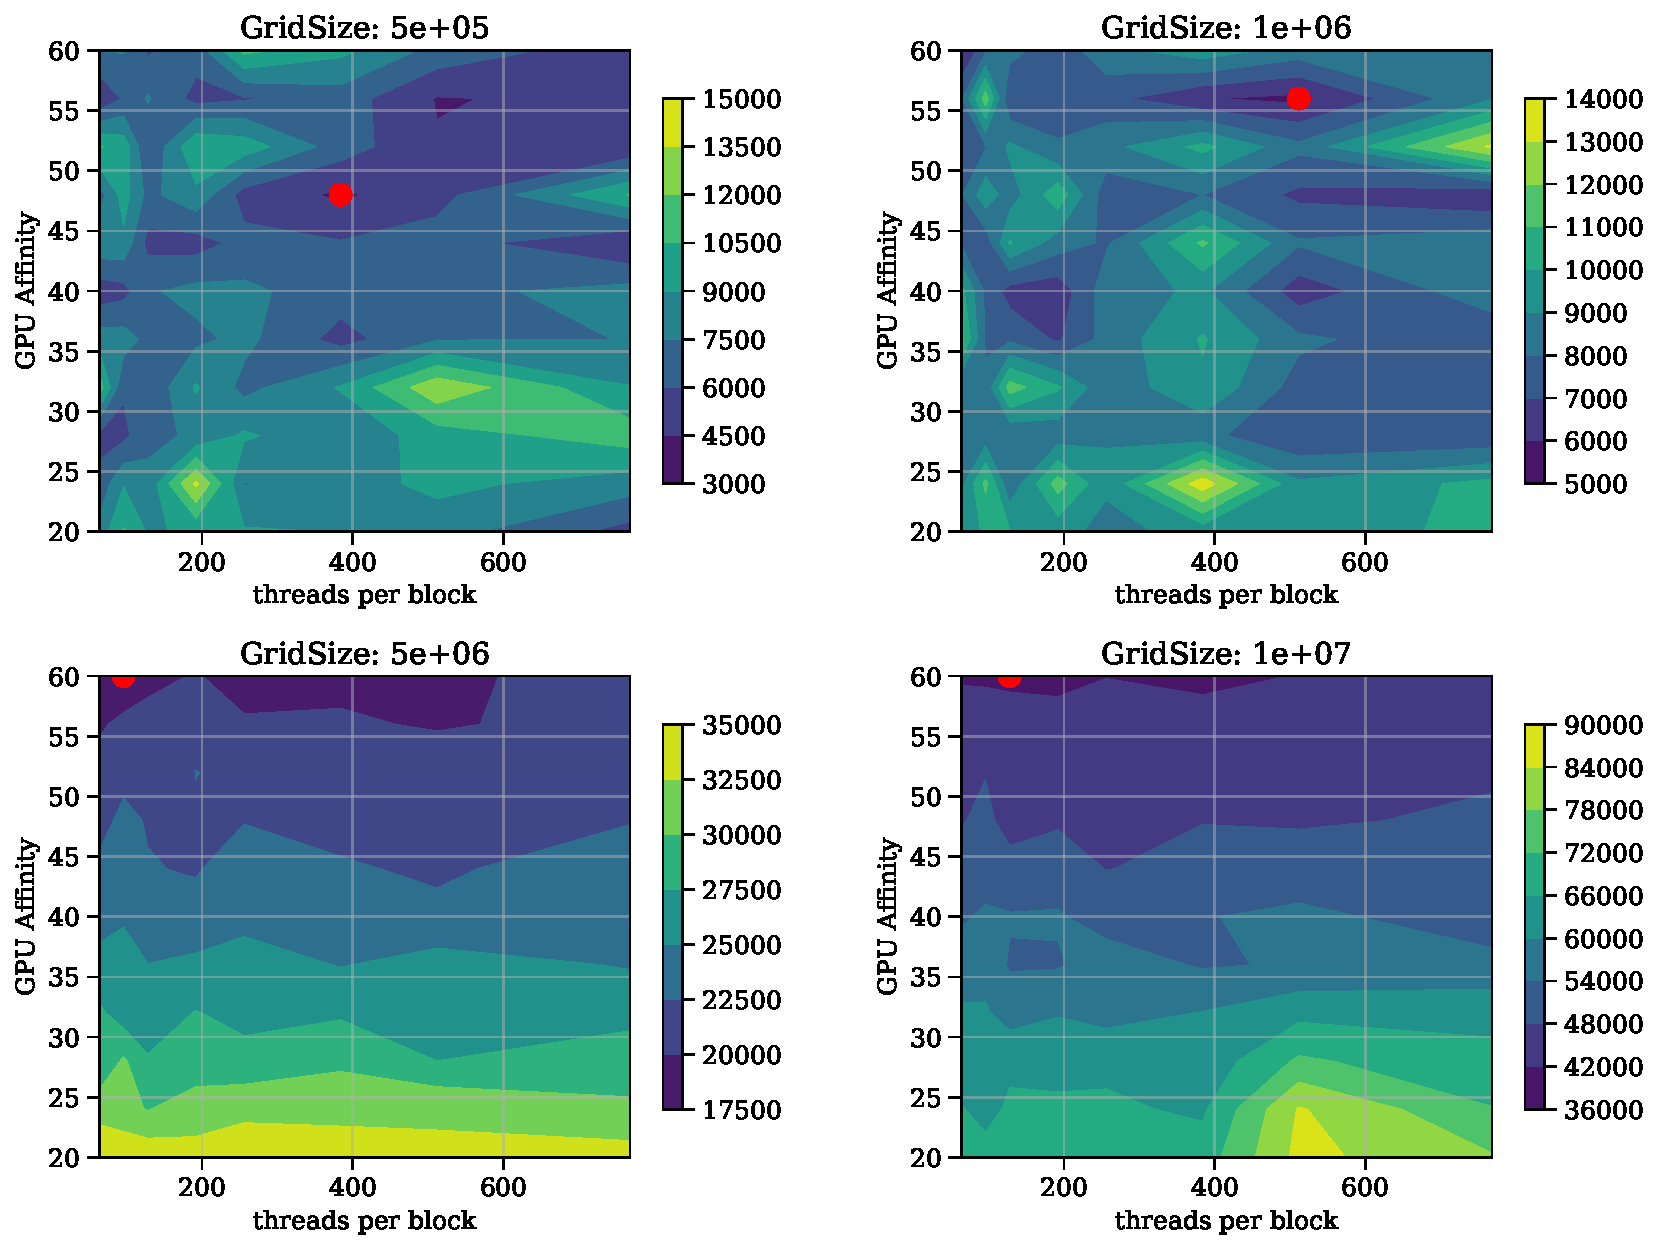
\includegraphics[width=\textwidth]{RawContourEulerClassictime}
        \caption{Classic decomposition}
        \label{f:EulerContourC}
    \end{subfigure}
    \begin{subfigure}[!tb]{.75\textwidth}
        \centering
        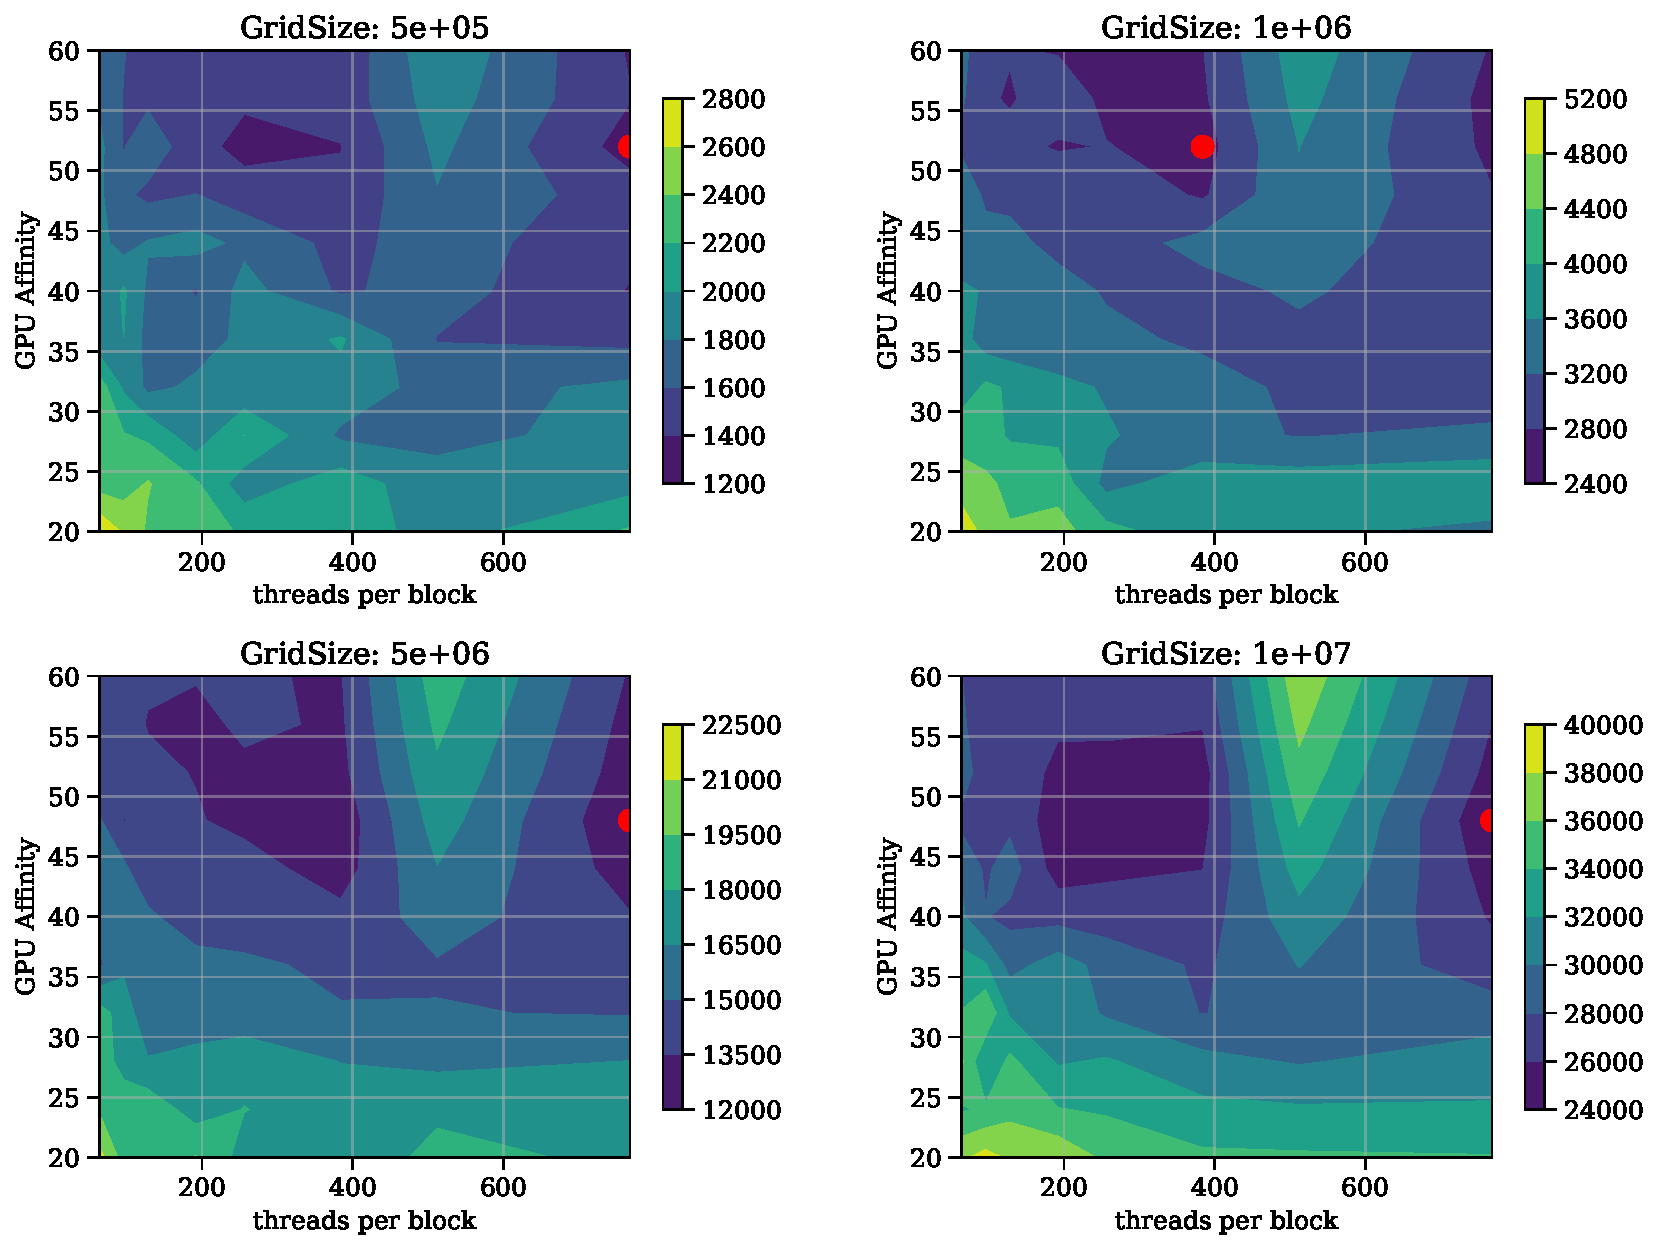
\includegraphics[width=\textwidth]{RawContourEulerSwepttime}
        \caption{Swept decomposition}
        \label{f:EulerContourS}
    \end{subfigure}
    \caption{A map of the time cost per timestep of the Euler equations at 4 grid sizes.
    The red dot signifies the best performance.}
    \label{f:EulerContours}
\end{figure}

\begin{figure}[htbp]
    \centering
    \begin{subfigure}[t]{.75\textwidth}
        \centering
        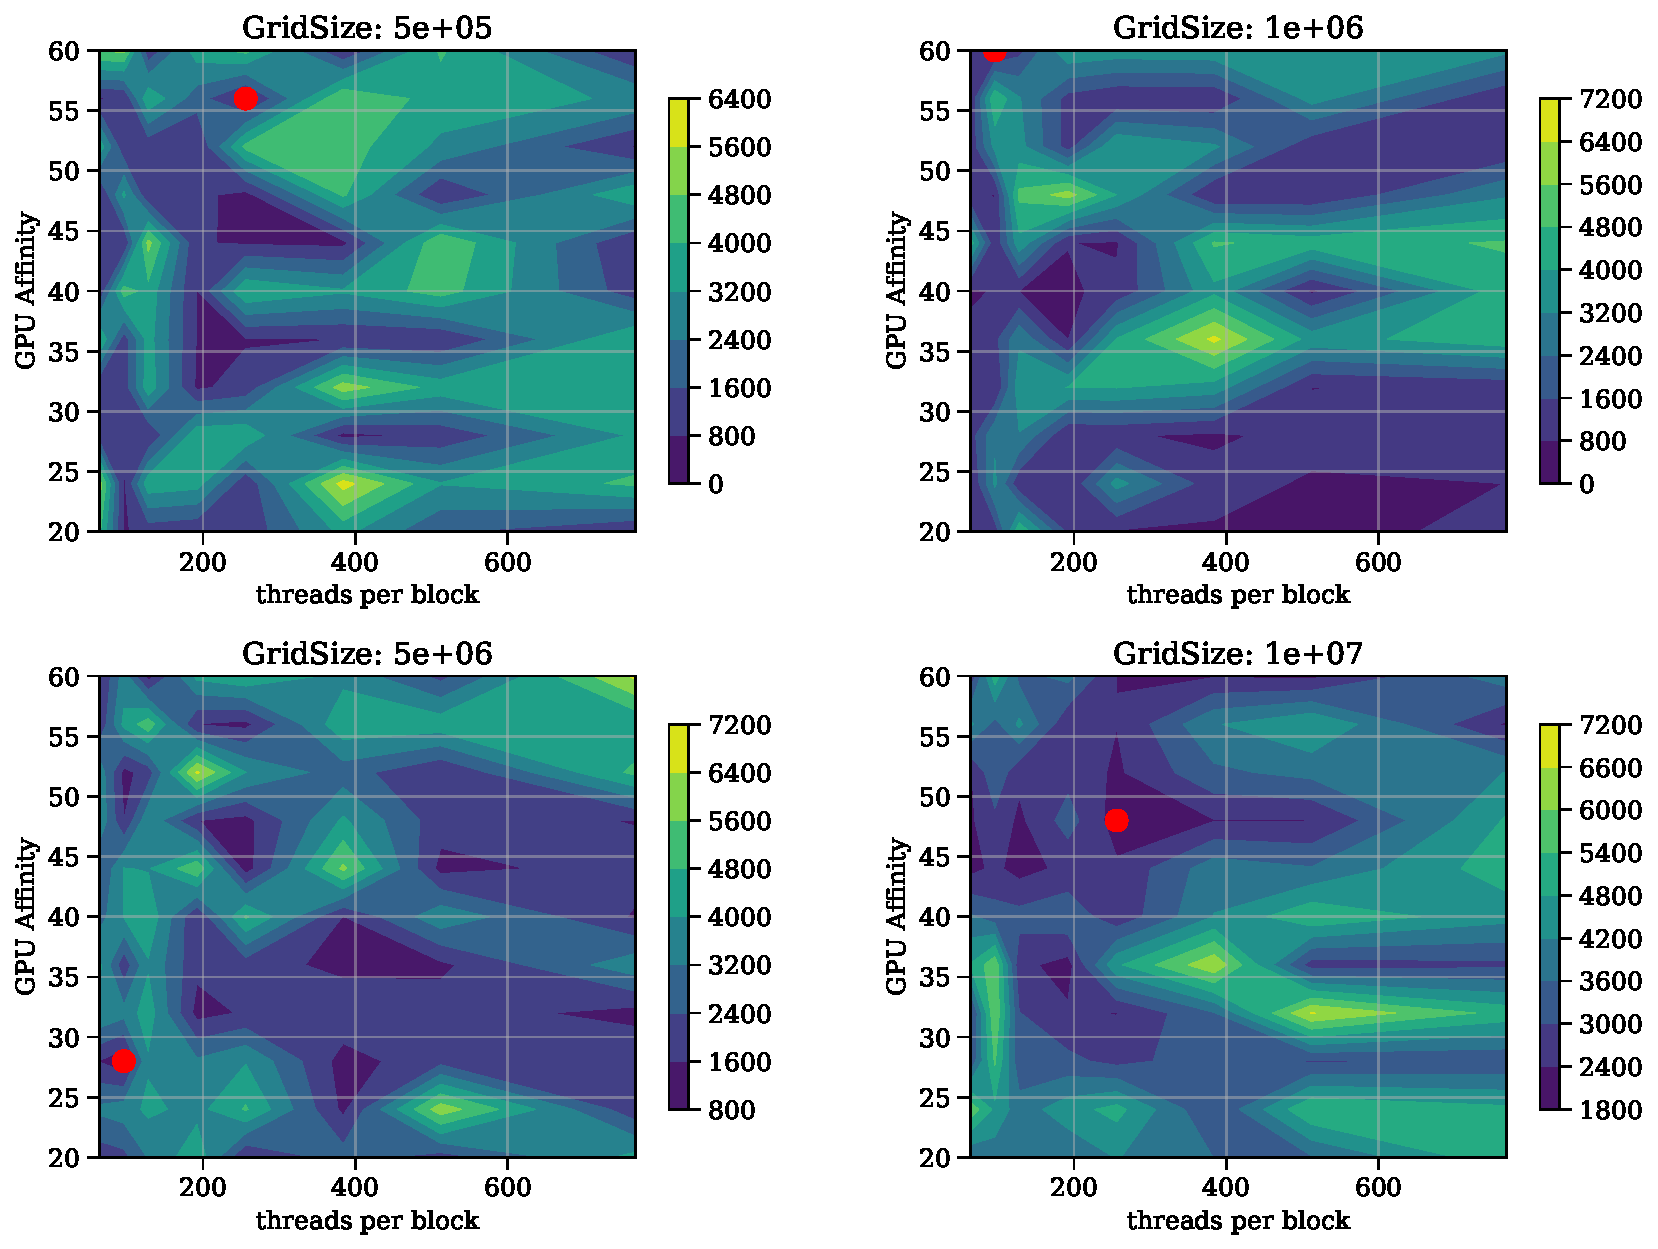
\includegraphics[width=\textwidth]{RawContourHeatClassictime}
        \caption{Classic decomposition}
        \label{f:HeatContourC}
    \end{subfigure}
    \begin{subfigure}[!tb]{.75\textwidth}
        \centering
        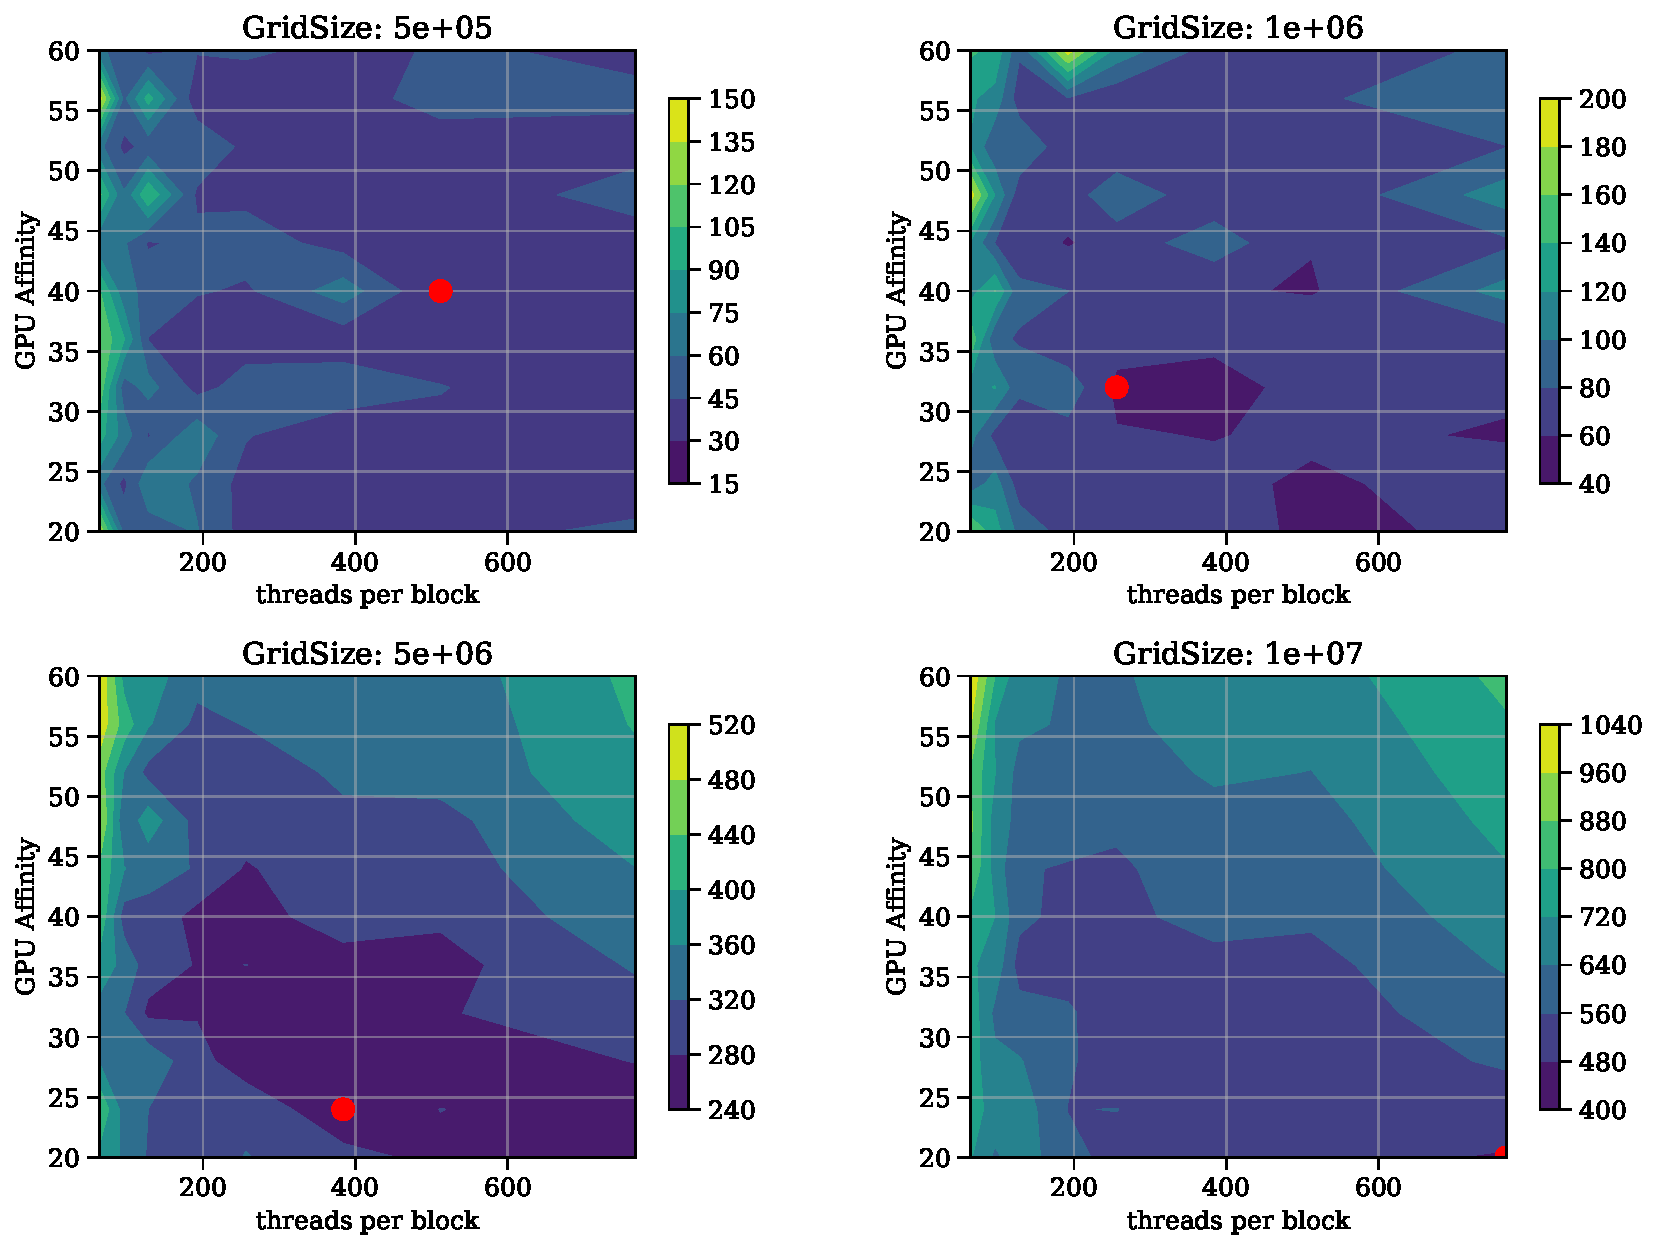
\includegraphics[width=\textwidth]{RawContourHeatSwepttime}
        \caption{Swept decomposition}
        \label{f:HeatContourS}
    \end{subfigure}
    \caption{A map of the time cost per time step of the heat equation at 4 grid sizes.
    The red dot signifies the best performance.}
    \label{f:HeatContours}
\end{figure}

Though we would emphasize that these results are representative of narrow experimental conditions,
architectures and design settings, the regularity of the \texttt{Swept} program performance
allows us to present fitted results in Table~\ref{tab:tablefit}, corresponding to the data points presented in Figures~\ref{f:BestRuntimeHeat} and ~\ref{f:BestRuntimeEuler}, that may illuminate and
guide future work on this and similar topics.

\begin{table}
\caption{Coefficients for power-law fit of grid size vs time per timestep ($y = Ax^b$) of \texttt{Swept} performance at best runtime configuration.}
%\vspace{-0.5em}
\label{tab:tablefit}
        \begin{center}
                \begin{tabular}{@{}l c c c}
                \toprule
                Equation & A & b & $R^2$ \\
                \midrule
                Euler   & \num{3.55e-3} & \num{0.976} & \num{0.999} \\
                Heat    & \num{1.08e-4} & \num{0.949} & \num{0.999} \\
                \bottomrule
                \end{tabular}
        \end{center}
\end{table}
